\documentclass[a4paper, 10pt, conference]{ieeeconf}      

% This command is only needed if you want to use the \thanks command
\IEEEoverridecommandlockouts                              
\overrideIEEEmargins
% See the \addtolength command later in the file to balance the column lengths
% on the last page of the document


%\usepackage{graphics} % for pdf, bitmapped graphics files
%\usepackage{epsfig} % for postscript graphics files
%\usepackage{mathptmx} % assumes new font selection scheme installed
%\usepackage{times} % assumes new font selection scheme installed
%\usepackage{amsmath} % assumes amsmath package installed
%\usepackage{amssymb}  % assumes amsmath package installed
\usepackage{comment}

\title{\LARGE \textbf{Capita selecta: AI Topics} \\ 
Automatic Statistician}


\author{Rick van Hek, Mathias Van Herreweghe}


\usepackage[T1]{fontenc}
\usepackage{graphicx}
\usepackage{lipsum}
\usepackage{verbatim}
\usepackage{amsbsy}
\usepackage{amsmath}
\usepackage{amsfonts}
\usepackage[colorinlistoftodos]{todonotes}
\let\proof\relax
\let\endproof\relax
\usepackage{amsthm}
\newtheorem{theorem}{Theorem}

\begin{document}

\maketitle
\thispagestyle{empty}
\pagestyle{empty}


%%%%%%%%%%%%%%%%%%%%%%%%%%%%%%%%%%%%%%%%%%%%%%%%%%%%%%%%%%%%%%%%%%%%%%%%%%%%%%%%
\begin{abstract}
    TODO: abstract, doen we dit voor zo een korte paper?
\end{abstract}

\tableofcontents
%%%%%%%%%%%%%%%%%%%%%%%%%%%%%%%%%%%%%%%%%%%%%%%%%%%%%%%%%%%%%%%%%%%%%%%%%%%%%%%%


\section{Introduction}
\section{The Automatic Statistician}
Interpreting data is not convenient without a model representing it. Due to the fact that making this model is rather time intensive, people have devoted time to automate this. Not only making a more visually appealing model, but also generating natural language descriptions about the model. In this paper we will mainly be describing the early system: \textit{Automatic Bayesian Covariance Discovery (ABCD)} described by Lloyd~\cite{lloyd2014automatic}. His system describes an open-ended language of Gaussian process models through a compositional grammar. Because of this compositional structure of the grammar, the system allows a way to generate natural-language descriptions of the structure. \\

A Gaussian process will model a distribution over multiple functions. Think of it as this way; if you have data, and you want to automatically find a function describing this data, you don't really know how many parameters you need. You want a way of not having to specify how many parameters the function should have. For example if you have a set of data points, you can model them by a very `spikey' function, such as in figure~\ref{fig:examplediagram}. But a better model would be a smoother function such as in figure~\ref{fig:examplediagram_vloeiend}. But this would require a lot more parameters.

\begin{figure}[!ht]
    \centering
    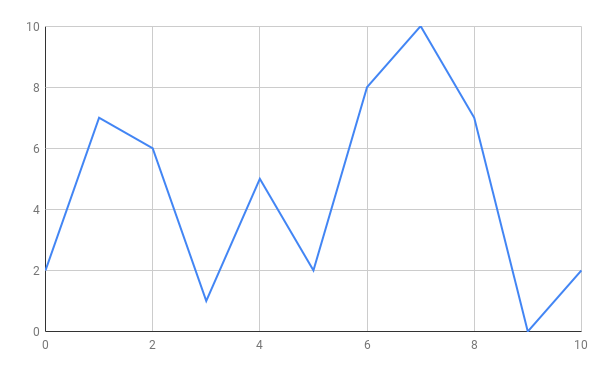
\includegraphics[width=0.6\linewidth]{report/images/examplediagram.png}
    \caption{}
    \label{fig:examplediagram}
\end{figure}
\begin{figure}[!ht]
    \centering
    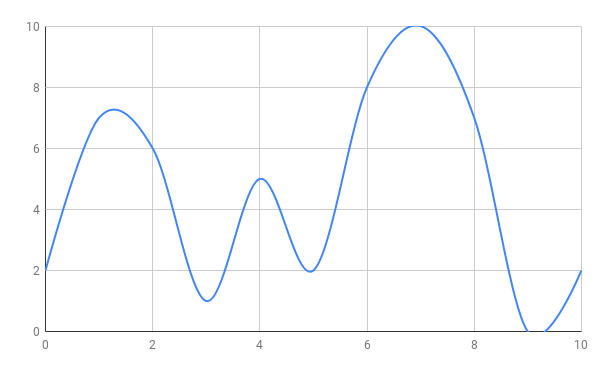
\includegraphics[width=0.6\linewidth]{report/images/examplediagram_vloeiend.png}
    \caption{}
    \label{fig:examplediagram_vloeiend}
\end{figure}

That's why GP's (Gaussian processes) are non-parametric, and have only two inputs: a mean function (\ref{eq:meanfunction}) and kernel (or covariance) function (\ref{eq:kernelfunction}). This mean- and kernel function will ensure this `smoothness'.

\begin{equation}\label{eq:meanfunction}
    \mu (x) = \mathbb{E}(f(x))
\end{equation}


\begin{equation}\label{eq:kernelfunction}
    k(x,x') = Cov(f(x), f(x'))
\end{equation}

The kernel function depicts a sort of similarity measure. If x and x', which are two input values, are close to each other, we expect the output to be close to each other as well. This will make sure the output is not too `spikey'.

So when a Gaussian Process is given (with a kernel and mean function), one can calculate the marginal likelihood of given data. You can also get a predictive distribution for new points, if you have already have existing data.

\subsection{The kernels}
This open-ended language contains multiple kernels in it's grammar, each describing a certain `feature' of a possible function. ABCD supports five different kernels that each encode something else:
\begin{itemize}
    \item White Noise (WN): uncorrelated noise
    \item Constant (C): constant functions
    \item Linear (LIN): linear functions
    \item Squared Exponential (SE): smooth functions
    \item Periodic (PER): periodic functions
\end{itemize}

ABCD further supports two compositional rules, that allow us to combine kernels and make more complex kernels. We have a rule to add (\ref{eq:compositionalrule_addition}) and multiply (\ref{eq:compositionalrule_multiply}) kernels.

\begin{equation}
    \label{eq:compositionalrule_addition}
    (k_1 + k_2)(x, x_0) = k_1(x, x_0) + k_2(x, x_0)
\end{equation}

\begin{equation}
    \label{eq:compositionalrule_multiply}
    (k_1 \times k_2)(x, x_0) = k_1(x, x_0) \times k_2(x, x_0)
\end{equation}

For example one could combine the Squared Exponential ($SE$) kernel with the Periodic ($PER$) kernel by multiplying these ($SE \times PER$), which will yield a kernel to approximate periodicity in the model.

One more operator has been added to the grammar, allowing change points to be incorporated. This is essential especially in Time Series data. Because the behavior of data could suddenly drastically change, such as in figure~\ref{fig:changepointexample}.
Changepoints are defined through addition and multiplication with sigmoidal functions:


\begin{equation}
    \label{eq:changepoint_1}
    \boldsymbol{CP}(k_1, k_2) = k_1 \times \boldsymbol{\sigma} + k_2 \times \boldsymbol{\bar{\sigma}}
\end{equation}

Where $\boldsymbol{\sigma} = \sigma(x)\sigma(x')$ and $\boldsymbol{\bar{\sigma}} = (1 - \sigma(x))(1 - \sigma(x'))$

\begin{figure}[ht!]
    \centering
    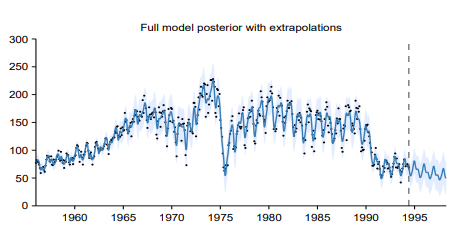
\includegraphics[width=\linewidth]{report/images/timeserieschangepoint.png}
    \caption{Example of a change point for time series data in the year 1710.~\cite{theautomaticstatistician:solar}}
    \label{fig:changepointexample}
\end{figure}

The base kernels have been expanded and reparameterised to allow for easier automatic translation to natural language description. These can be seen in table~\ref{tab:regressionmodelkernel}

\begin{table}[]
\begin{tabular}{ll}
Regression model                                & Kernel                    \\ \hline
\multicolumn{1}{l|}{GP smoothing}               & $SE + WN$                 \\
\multicolumn{1}{l|}{Linear regression}          & $C + LIN + WN$            \\
\multicolumn{1}{l|}{Multiple kernel}            & $\sum SE + WN$            \\
\multicolumn{1}{l|}{Trend, cyclical, irregular} & $\sum SE + \sum PER + WN$ \\
\multicolumn{1}{l|}{Fourier decomposition}      & $C + \sum cos + WN$       \\
\multicolumn{1}{l|}{Sparse spectrum GPs}        & $\sum cos + WN$           \\
\multicolumn{1}{l|}{Spectral mixture}           & $\sum SE \times cos + WN$ \\
\multicolumn{1}{l|}{Changepoints}               & e.g. $CP(SE, SE) + WN$    \\
\multicolumn{1}{l|}{Heteroscedasticity}         & e.g. $SE + LIN \times WN$
\end{tabular}
\caption{Common regression models expressible in their language. \textit{cos} is a special case of the reparametrised \textit{PER}~\cite{lloyd2014automatic}}
\label{tab:regressionmodelkernel}
\end{table}

\subsection{Searching for a model and evaluate}
TODO

\subsection{Automatic natural language description generation}
TODO (weet niet of dit wel echt moet, lijkt me niet echt belangrijk voor ons project)

\section{Creative part}
The Automatic Statistician's website \todo{link to website here} contains examples of demo runs of the software. The examples are the reports generated by the Automatic Statistician. We will replicate a manual machine learning procedure for two of the examples and compare our results to those of the report. We will make such a comparison for the affairs dataset \todo{ref to dataset} in subsection \ref{subsec:reg_affairs} and the airline passengers dataset \todo{ref to airl pass dataset} in subsection \ref{subsec:ts_airpas}.

\subsection{Regression: affairs}
The affairs dataset consists of multiple variables, these are the gender of a person, the amount of years married, whether or not a person has children, the degree of religiousness, the level of education, the kind of occupation (higher number means more prestigious) and the rating of a person's relationship. The target variable is the amount of extra-marital affairs the person had. The gender and children variable were excluded from the Automatic Statistician's input, as these were the non-numeric variables, so we did the same.\\

The Automatic Statistician performs a regression analysis by comparing three simple strategies for linear models using 5 fold cross validation on half of the data. The strategy with the lowest cross validated prediction error has then been used to train a model with the same half of data. The results of the regression can be found in table \ref{table:as_affairs}, the result is expressed as the root mean squared error (RMSE) of the cross validation.

\begin{table}[!h]
\centering
\begin{tabular}{| l | l |}
  \hline
  Method & Cross validated RMSE \\
  \hline
  Full linear model & 3.22 \\
  BIC stepwise & 3.31 \\
  LASSO & 3.33 \\
  \hline
\end{tabular}
\caption{Results regression analysis Automatic Statistician}
\label{table:as_affairs}
\end{table}

Another part of the analysis is that it gives a summary of the relation between variables and the target variable. It finds that the output affairs

\begin{itemize}
    \item decreases linearly with input rating (correlation $-0.25$),
    \item decreases linearly with input religiousness (correlation $-0.22$),
    \item increases linearly with input years married (correlation $0.16$),
    \item decreases linearly with input age (correlation $0.10$),
    \item increases linearly with input occupation (correlation $0.12$),
    \item decreases linearly with input education (correlation $0.04$).
\end{itemize}

The report then concludes with a critical evaluation of its used model, which we will not further discuss in this report.\\

We then took it to ourselves to produce a model that would yield a better score than that of the Automatic Statistician. We started by exploring the data. We searched for outliers in the data using scatterplots and boxplots for all variables. We did not see the need to prune or correct anything within the data based on these plots. We created two new variables, these are \textit{marriageScore} which is the number of years married times the rating of the marriage, and \textit{experienceScore}, which is the age times the level of education times the kind of occupation. We then did a correlation analysis on the variables to find which were correlated the most to the output, these correlations can be found in table \ref{table:correlation_affairs}.

\begin{table}[!h]
\centering
\begin{tabular}{| l | l |}
  \hline
  Variable & Correlation score \\
  \hline
  yearsmarried &      0.187 \\
  age &               0.095 \\
  experienceScore &   0.076 \\
  occupation &        0.050 \\
  marriageScore &     0.037 \\
  education &        -0.002 \\
  religiousness &    -0.145 \\
  rating &           -0.280 \\
  \hline
\end{tabular}
\caption{Results correlation analysis}
\label{table:correlation_affairs}
\end{table}

We then create additional variables based on the three most correlated variables. We include the square, cube and square root of variables \textit{yearsmarried}, \textit{age} and \textit{experienceScore}. Subsequently we create different models and compare the root mean squared error in the same manner the Automatic Statistician did. The results of the regression analysis can be found in table \ref{table:results_affairs}.

\begin{table}[!h]
\centering
\begin{tabular}{| l | l | l |}
  \hline
  Method & RMSE & RMSE* \\
  \hline
  Gradient Boosting Method & 3.75 & 3.68 \\
  Random Forest & 3.25 & 3.23 \\
  LASSO & 3.12 & 3.10 \\
  ElasticNet & 3.17 & 3.11 \\
  Kernel Ridge & 3.16 & 3.30 \\
  Support Vector Regression & 3.44 & 3.68 \\
  \hline
\end{tabular}
\caption{Results regression analysis, rounded to 2 decimals (* original variables only, as used by Automatic Statistician)}
\label{table:results_affairs}
\end{table}
\todo[inline]{Add refs to models in table above}

As can be seen, some models score better than the model with the lowest RMSE of Automatic Statistician. Another part of Automatic Statistician's report that we wanted to try to replicate or even improve upon was explore the relationship between the variables and the output. We did this exploration by means of partial dependence plots.
\todo{partial dependence plots}

\label{subsec:reg_affairs}
% TODO
\subsection{Time series: airline passengers}
\label{subsec:ts_airpas}
% TODO

\subsection{Summary}
\label{subsec:summary_creative_part}
% short conclusion / remark on AS' skills

\section{Conclusion}
TODO
What have we learned?....


\addtolength{\textheight}{-12cm}  

\bibliography{references}
\bibliographystyle{IEEEtran}

\end{document}
